% !TEX root=../main.tex
\documentclass[beamer]{standalone}
\begin{document}
% ===========================================
% Results - Video
% ===========================================
\begin{frame}{Results}
    \framesubtitle{Video}

\note[item] {
    Here is the video result.
}

\end{frame}

% ===========================================
% Results - Analysis
% ===========================================
% \begin{frame}{Results}
% \framesubtitle{Shape reconstruction comparison}
%     \begin{figure}
%         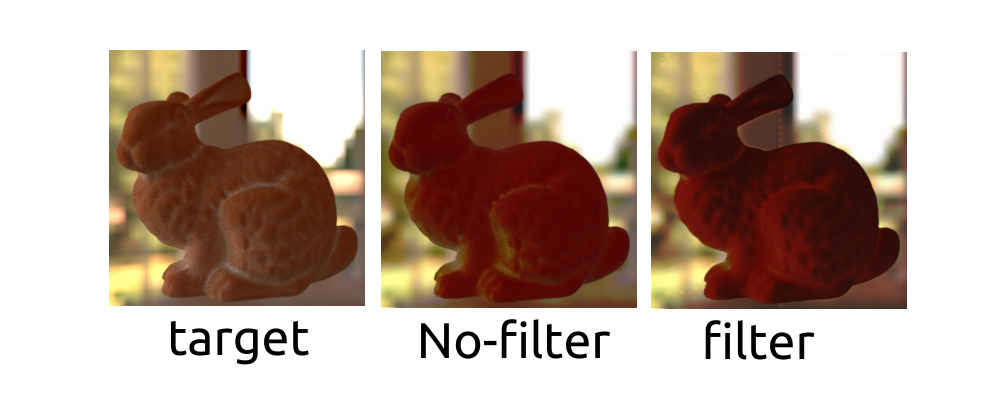
\includegraphics[height=0.85\textheight]{figures/result-3.png}
%     \end{figure}

% \note[item] {
%     This is the comparison result of inverse shape reconstruction.
% }

% \end{frame}

% ===========================================
% Results - Texture
% ===========================================
\begin{frame}{Results}
\framesubtitle{Texture reconstruction using Monte Carlo sampling}
    \begin{figure}
        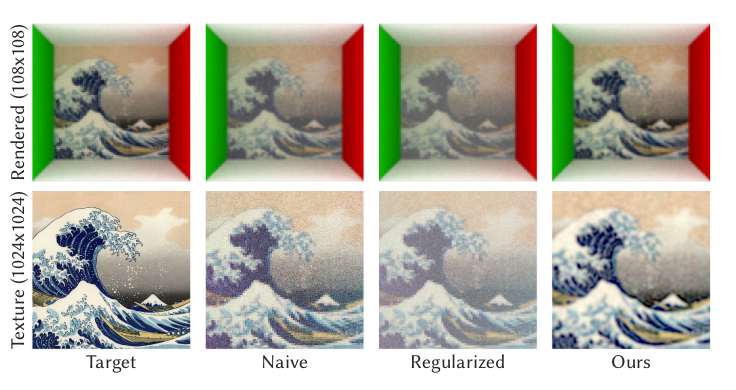
\includegraphics[width=0.8\textwidth]{figures/result-4.png}
    \end{figure}

    % note %
\note[item]{
    % @@TODO
    Also, the authors suggest another adaption of this second-order derivative method.

    The suggested example is texture reconstruction in Monte Carlo rendering.

    Because of the noisy gradient, we should take small steps on this optimization sequence or need some regularaization in differentiable path tracing.
    Their method can solve this problem as the point of view on filtering the gradient.
}
\end{frame}
\end{document}